\chapter[Chopin and Prelude, Op. 28, No. 15]{Frédéric Chopin - \textit{Prelude, Op. 28}, No. 15, the ``Raindrop'' Prelude (1838)}

Fryderyk Chopin (1810-1849) was a composer during the Romantic period (generally known to be from 1800-1910) who composed primarily for the piano. Born near Warsaw in a section of Poland which was at the time under Russian control, Chopin's clear talents as a musician were clear from an early age. By age seven, he had played his first public concert as a soloist, and had published his first piece. Over the course of years, his pieces would evolve to have a defined Polish character. In 1830, Chopin began touring through Germany and Italy, to gain an international reputation as a performer and composer, and settled in Paris, France in 1831. By this point, Chopin had already mostly reached fully compositional maturity. Four genres generally attributed to Chopin, the mazurka, étude, waltz, and polonaise, had matured by then, as Chopin had begun writing these in the 1820s\autocite{Burkholder_Grout_Palisca_2014}. The étude, a genre heavily associated with both Chopin and fellow Romantic-era composer Franz Liszt, is a piece which is intended to develop technique, or a certain skill on the instrument of choice, and only develops a singular figure through the piece. The other three genres that are known to be \say{Chopin genres} are stylized dances, typically for students, and are idiomatic in both figurations and fingerings\autocite{Burkholder_Grout_Palisca_2014}. Chopin's waltzes evoked the spirit of ballrooms in Vienna, but the mazurkas and polonaises are infused with Polish character. The polonaise is a type of courtly, and aristocratic dance, in $\frac{3}{4}$ time, also marked by a rhythmic figure of one eighth note and two sixteenth notes on beat one. The mazurka is a Polish folk dance, and in the time of Chopin, had become an urban type of ballroom dance, popular amongst those in high society in both Paris and Poland. Similar to the polonaise, the mazurka is in $\frac{3}{4}$ time, with accents on beats two or three, and a dotted figure of some kind on beat one. Mazurkas also feature a simple accompaniment, especially in the left-hand for piano, and combine four-bar long phrases into periods which alternate in A BA C form. The melody for a mazurka is also important, as it is instrumental in style, rather than vocal in style. This leads to elements of Polish instrumental folk music being prominent, and includes aspects solely found in melodies of instrumental music: large trills, grace notes, large leaps from one note to the next, and slurs to imitate the bowing found in traditional Polish folk songs. If articulated properly, a mazurka would sound uneven in tempo as it allows for ornamentations (such as the \textit{sforzando}, trills, and grace notes) to lengthen in time, and would lead to dancers to be able to execute turns or lifts. 

In the years before 1838, when the Raindrop Prelude was written, there was a brief, albeit interesting, period of Chopin's life. A period of writing, 1837 marked the year in which Chopin crossed paths with George Sand, a novelist later to be Chopin's partner, yet it was not until April 1838 in which they made this pairing official. The pair, along with Sand's children, spent the winter months of 1838-9 in Valldemossa, Majorca, an old Carthusian monastery. Recuperating from an illness and in the midst of a winter storm, Chopin began writing the 24-set preludes\autocite{Samson_2001}. Thus, the title of the fifteenth prelude of this set relates to the rain and stormy weather Chopin weathered while at Majorca, as well as the uncertainty regarding his health, of which the second point will be expanded upon in section \ref{subsection:chopin-intepretation}.

In 1838, Chopin wrote the set of 24 preludes, Opus 28, of which the fifteenth (simply known as the \say{Raindrop Prelude} is arguably one of the most famous of this set. Structurally, this prelude is in ternary form, with three sections: \textit{ABA}, and a coda. 

\begin{figure}
  \centering
  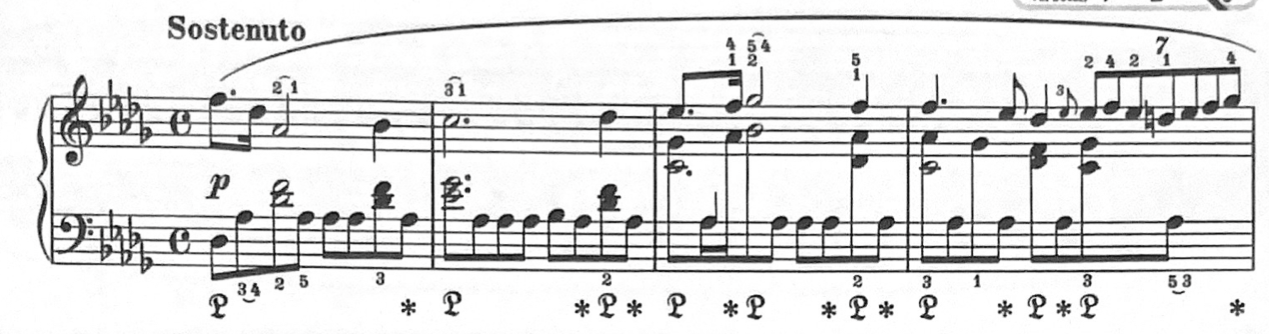
\includegraphics[width=\textwidth]{chopin-a-section-first-four-bars.jpg}
  \caption{The first four bars of Chopin's \textit{Prelude, Op. 28, No. 15}}
  \label{fig:chopin-a-section-first-four-bars}
\end{figure}

\begin{figure}
  \centering
  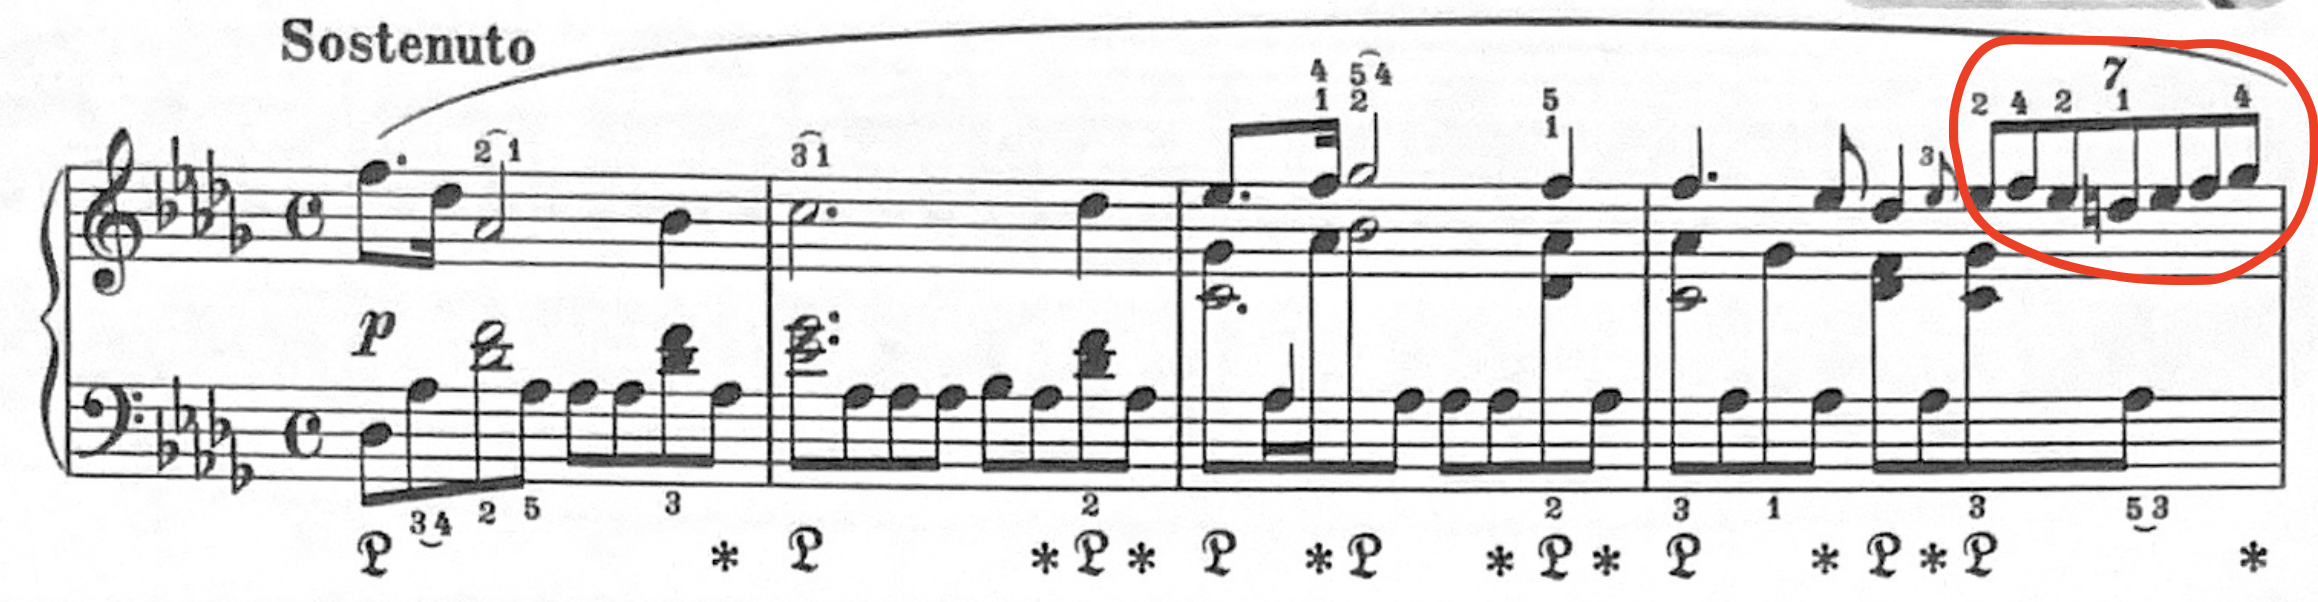
\includegraphics[width=\textwidth]{chopin-a-section-seven-note-run.jpg}
  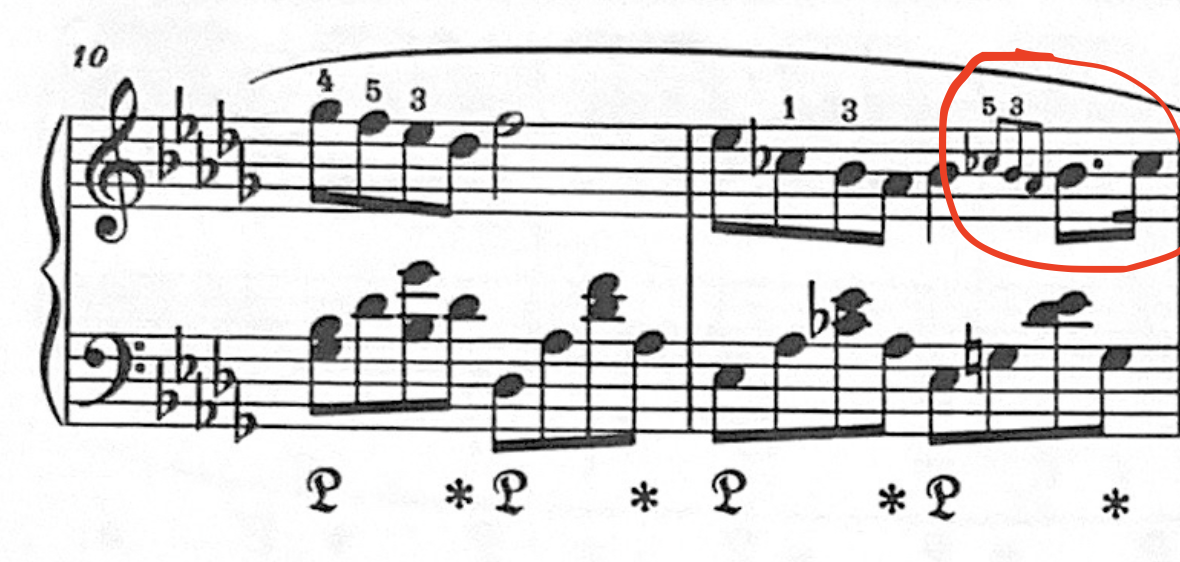
\includegraphics[width=\textwidth]{chopin-a-section-triplet-grace-note.jpg}
  \caption{Several examples of ornamentation, in Chopin's \textit{Prelude, Op. 28, No. 15}}
  \label{fig:chopin-a-section-examples-ornamentation}
\end{figure}

The first section, A, is a sweet section, reminiscent of gentle rain, akin to a sprinkle of rain. The delicate nature of this section is shown in the continuous usage of the \textit{piano} dynamic, as in Figure \ref{fig:chopin-a-section-first-four-bars}\autocite{Hansen_1973}. So, the performer playing this piece will play this section, as well as its related A' section, as the most expressive of the piece. As implied in bars three and four of Figure \ref{fig:chopin-a-section-first-four-bars}\autocite{Hansen_1973}, this typically becomes an interpretation in which there is a consistent usage of \textit{rubato}\autocite{Cole_Schwartz}\footnote{A common practice in Romantic-era compositions. It involves taking a part of the duration of one note, and then giving it to another note. The performer is tasked with tastefully stretching, slowing, or hurrying the tempo, to their discretion. This gives the performer the greatest amount of flexibility and emotion available to interpret the piece.} and gradual crescendos and decrescendos to and from mezzo piano (medium loud). This is best seen when the piece in bars three and four ascend, peaking on the note G, and then descend, to a temporary low of D. This rise to G and subsequent fall to D will typically be played as a crescendo as the performer reaches the note G, and then a decrescendo back to \textit{piano} as the performer approaches the note D. The titular raindrop that this piece is named after is easily heard within the first three notes played in this piece and section: F, D\musFlat{}, and A\musFlat{}, outlining the piece's tonic key of D\musFlat{} Major. This phrase of three notes repeats again in other places in section A and A', as the raindrop motif, signifying the raindrops falling, and giving the section a melody which is cantabile and smooth. This section also features a repeated-note motif of the A\musFlat{} which is found in the left hand, as in Figure \ref{fig:chopin-a-section-first-four-bars}\autocite{Hansen_1973} and many other places throughout A and A' sections. The raindrop motif stands out more against the background hum, or the sounds of other raindrops falling in tandum, which the left hand's pedal point provides. The two motives here provide a texture which is entirely homophonic in this section. The texture solely consists of the right hand melody, and the raindrop motif, and the left hand's accompaniment, with the pedal point motive. This causes the section to sound thin in texture and timbre, as the right hand provides its melody through the use of broken chords, and the left hand provides a pedal note. Beyond the simplistic homophonic. texture, this section also contains tasteful ornamentations, featuring the use of rubato and other rhythmic ornamentations, among others, as shown by Figure \ref{fig:chopin-a-section-examples-ornamentation}. In the end of the A section, there is a key change to the relative minor key of C\musSharp{} Minor, D\musFlat{} Major's relative minor key. This becomes the B section's tonic key.

\begin{figure}
  \centering
  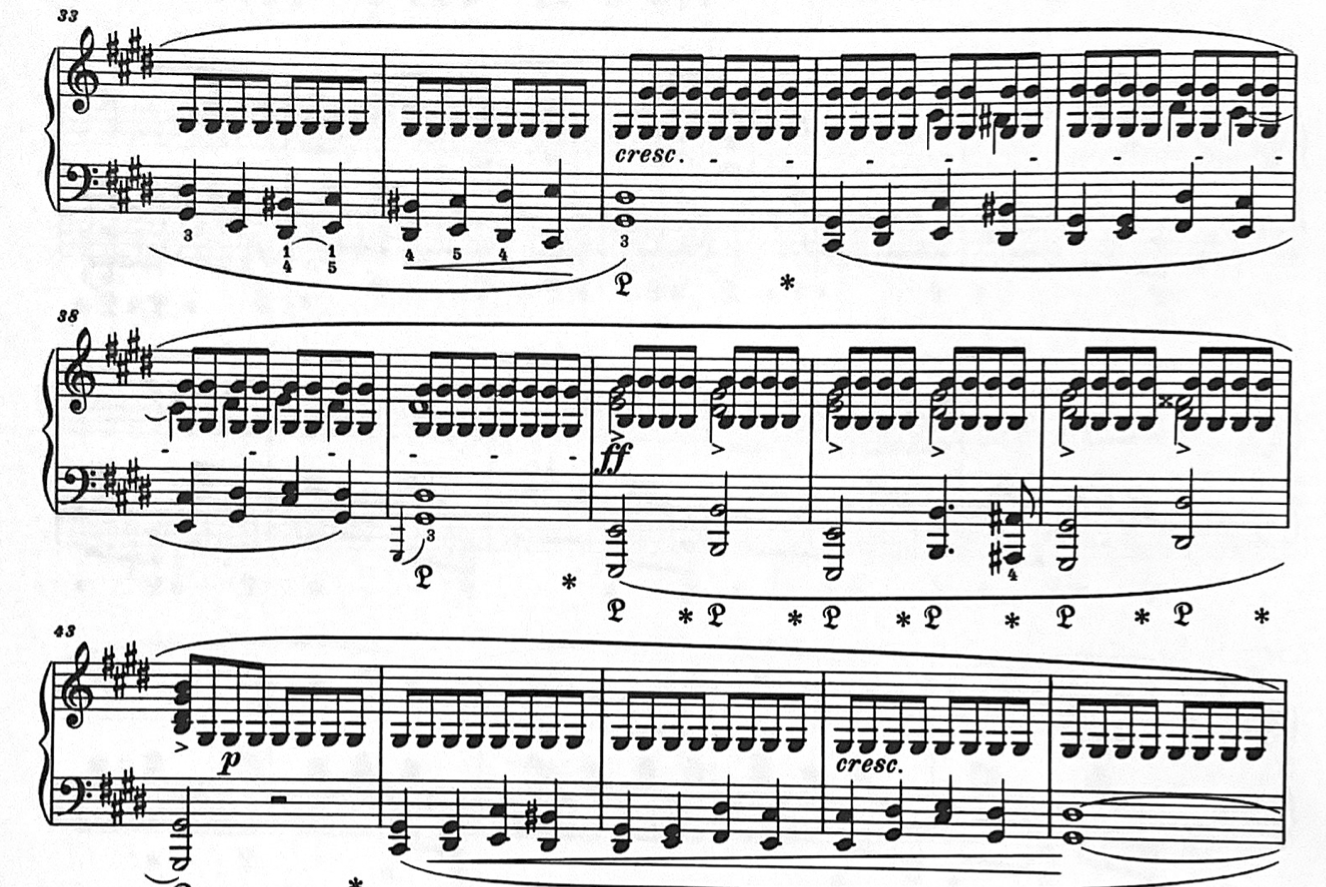
\includegraphics[width=\textwidth]{chopin-b-section-crescendos.jpg}
  \caption{The changes in dynamics, in Chopin's \textit{Prelude, Op. 28, No. 15}}
  \label{fig:chopin-b-section-crescendos}
\end{figure}

\begin{figure}
  \centering
  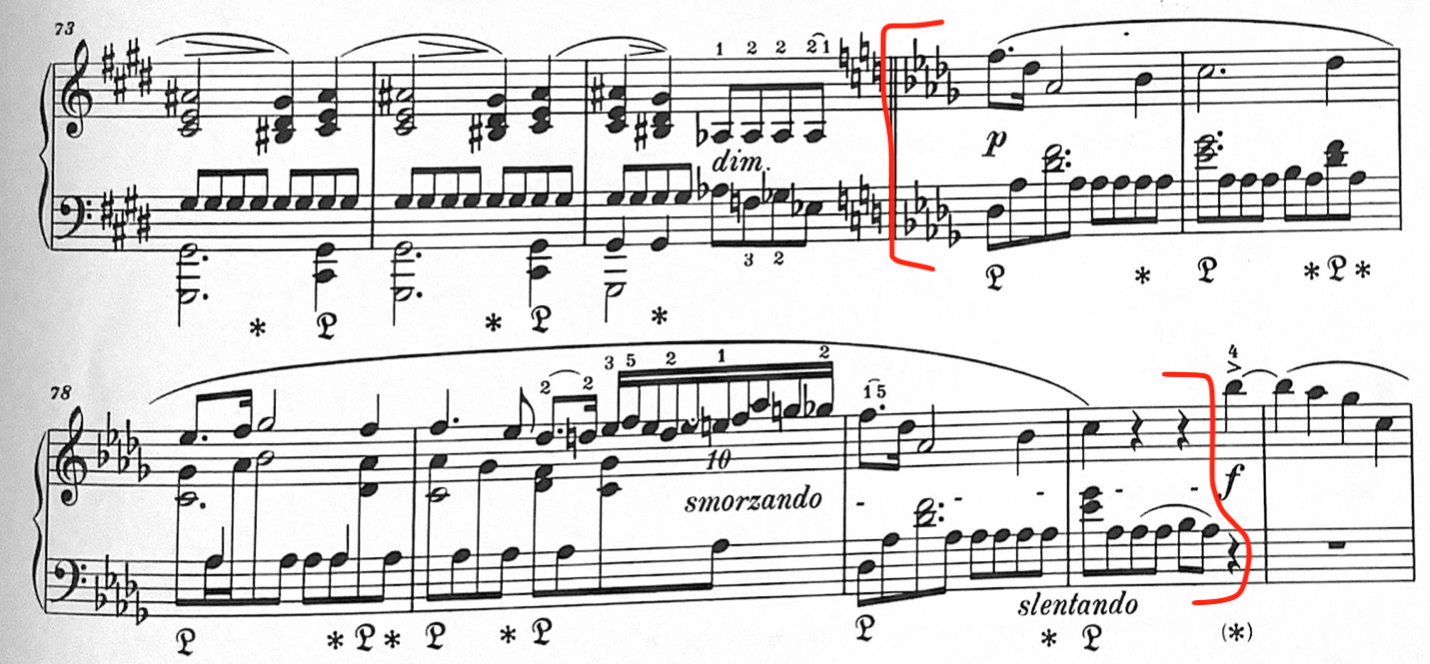
\includegraphics[width=\textwidth]{chopin-a-prime-section-ornamentation.jpg}
  \caption[Ornamentations in A', Chopin's \textit{Prelude, Op. 28, No. 15}]{The various ornamentations in the A' section of Chopin's \textit{Prelude, Op. 28, No. 15}}
  \label{fig:chopin-a-prime-section-ornamentation}
\end{figure}

\begin{figure}
  \centering
  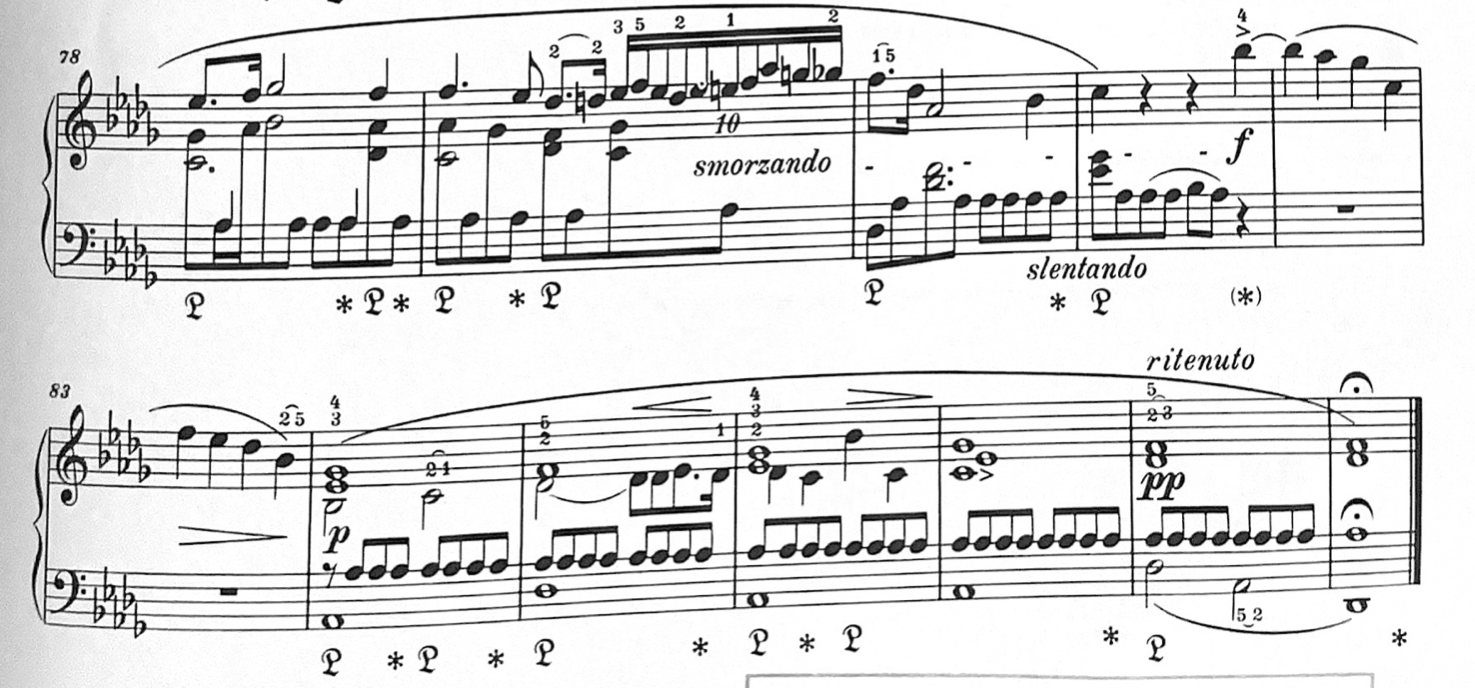
\includegraphics[width=\textwidth]{chopin-coda.jpg}
  \caption{The coda, Chopin's \textit{Prelude, Op. 28, No. 15}}
  \label{fig:chopin-coda}
\end{figure}



The B section is a high contrast to section A in character and tone. With the key change to C\musSharp{} Minor, the pedal note of A\musFlat{} turns into G\musSharp{}, and tension is introduced in this section. While section A's texture was a homophonic one, this section's texture is much more chordal, with chords featured in both hands, and also contains notes which are generally lower in pitch. Additionally, the repeated note motif is now in the right hand, as it plays the note G\musSharp{}, in Figure \ref{fig:chopin-b-section-crescendos}\autocite{Hansen_1973}, creating a sort of ``inverted'' pedal point. The melody then shifts to the left hand. As the section goes on, crescendos are used to build additional tension (see Figure \ref{fig:chopin-b-section-repeated-note-motif}\autocite{Hansen_1973} for reference, for example) as the dynamics increase from \textit{sotto voce} to \textit{fortissimo} ( \say{very loud}). The section begins \textit{sotto voce} (``under the voice'', which has similar meaning to \textit{piano}), and gradually builds with crescendos\footnote{Figure \ref{fig:chopin-b-section-crescendos}}\autocite{Hansen_1973}. As the tension builds, the left hand also adds slurs as ornamentation, adding a legato effect to the notes which also contributes to the rising tension. Once the dynamics peak at \textit{fortissimo}, the volume drops to \textit{piano} and repeats the section again. Dynamics are the primary tool used by the performer to add their interpretation and expression to the piece in this section, and the \textit{fortissimo} is used to great effect when the crescendo builds, and is at its highest when we arrive at the chords of E Major and B Major.

The return of the A section, although a modified version, returns the original melody of the first A section. It return \textit{piano}, and is also marked \textit{smorzando} (``dying away'') to signify the intended ending in \textit{pianissimo} (very soft). The first A section's tonic key of D\musFlat{} Major returns, and so does a majority of the ornamentation decisions, including rubato, and other decorations which are explored more deeply, as in Figure \ref{fig:chopin-a-prime-section-ornamentation}\autocite{Hansen_1973}. However, we only hear the first eight bars of this second A section, as Chopin includes a coda to finish the piece.

This coda (or more accurately, codetta, a short coda) finishes the prelude. As seen in Figure \ref{fig:chopin-coda}\autocite{Hansen_1973} and marked in red brackets, there are elongated quarter notes which descend, played in \textit{forte} (loud), to add a sense of both intensity and delicacy to the ending. In the third full bar of the coda, the pedal point is reintroduced, this time as A\musFlat{}, played in the right hand. It, like its role in the first A section, is like that of falling raindrops, serving as a background sprinkle for this ending. The coda ending is marked with the word \textit{ritenuto}\autocite{Cole_Schwartz_Ritenuto}, to indicate the sudden slowing of the tempo, almost an extreme slowing of the tempo. With the \textit{ritenuto}, it is a clear ending to this prelude, and is akin to the ending of a rainstorm, in which the rain clears up.

\section{Death on an Island}